\documentclass[main.tex]{subfiles}

\begin{document}
The output of the GEANT4 was used to fit the data spectra. 
First, however, it had to be processed. 

\section{Simulation Results Processing}
After the GEANT4 simulation was done, the output file had to processed further.  
Much like the experimental data, the simulated data had to be filtered.
This was done using the TTrees from the output files of the GEANT4 simulation.
The energy absorbed in the implant detector was filtered by the energy absorbed in the outer four gamma detectors in the simulation.

The two different categories of energy absorbed in the implant detector were built into two histograms. 
One histogram had a condition that the energy absorbed by the initial gamma ray had to be zero.
This histogram was the energy absorbed without any summing.
The second histogram was the energy absorbed where there was a contribution from the gamma ray.
This histogram was known as the energy absorbed with summing.
These two histograms can be seen in figure \ref{fig:GEANT4Hists}

\begin{figure}[!htb]
	\centerline{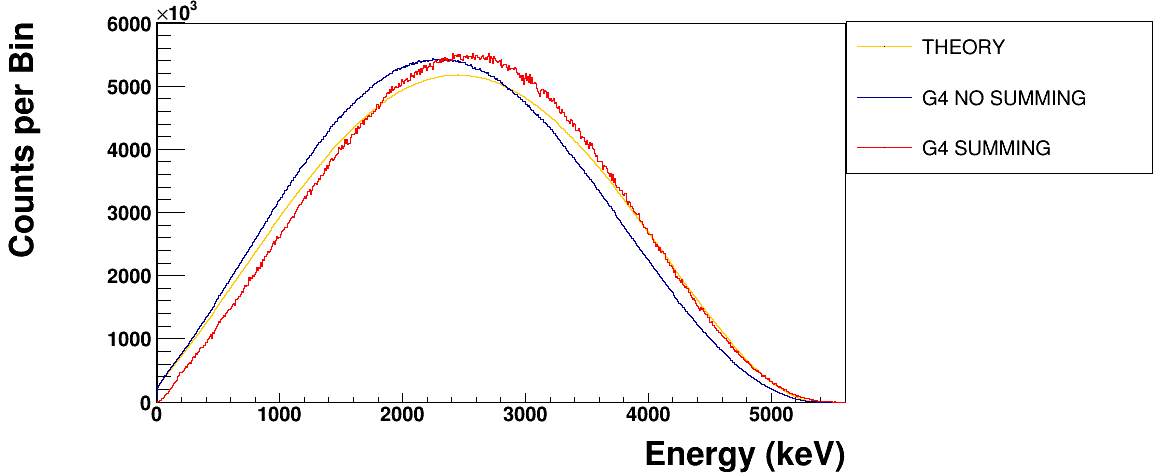
\includegraphics[width=0.78\textwidth]{GEANT4OutputBetter.png}}
	\caption{The shapes of the different histograms from the output of the GEANT4 simulation.
		 The input beta spectrum is also plotted.
		 The histograms are put to the same scale.}
	\label{fig:GEANT4Hists}
\end{figure}

\subsubsection{Detector Resolution}
\label{sec:convolution}
The next step was the apply the detector resolution to this histogram.
This was done by applying a convolution function to the histograms built from the GEANT4 output files.
The convolution function was

\begin{equation}
	\sigma = A\sqrt{E}
	\label{eq:convo}
\end{equation}

where $\sigma$ was the energy resolution, $E$ the energy, and $A$ a constant found through a calibration.
This was done by looping through each of the histograms bin by bin and reading the number of counts in each bin.
For each bin a Gaussian function was built.
The centroid of the Gaussian was the center of each bin in keV.
The $\sigma$ of the Gaussian was calculated by using equation \ref{eq:convo}.
This Gaussian function was sampled as many times as there were counts in the bin.
These samples were filled into a new histogram.
This was repeated bin by bin until all bins were distributed.

\subsubsection{Determining Detector Resolution}
In order to properly fit the energy spectrum, a calibration of the CsI(Na) detector had to be done.
The calibration was used to find what the detector resolution was.
Several different energy lines were used to find the calibration and the energy resolution function.
The lines were the 1.173228 MeV and 1.332492 MeV gammas from a $^{60}$Co source, the 0.661657 MeV gamma ray from a$^{137}$Cs source, and the 0.511 MeV and 1.274527 MeV gamma rays from a $^{22}$Na source.
These gamma rays were fitting with a Gaussian and a background.
The background varied from a linear background, a quadratic background, and an error function background.
For the $^{60}$Co, both peaks were fit at once.
These different background gave slightly different results for the centroids and the widths of the Gaussian.
The different widths and centroids were taken as a systematic error.
From the centroids, the calibration for each detector was calculated and shown in equation \ref{eq:cal}

\begin{equation}
	C = G * E + b
	\label{eq:cal}
\end{equation}

where $C$ is the location of the peak in ADC channels, $G$ the gain in channels/keV, and b the offset in channels.
This calibration curve was only used for the resolution determination.
The widths of the peaks were calibrated with the gain and plotted vs energy.
Then, equation \ref{eq:convo} was fit to the results in order to determine $A$.
The value of $A$ used for this procedure was 1.118.

\subsubsection{Pile-up Modeling}
After the convolution, the simulation data was sent through a simulation to model pile-up.
The model used for the CsI(Na) signals was a linear rise and then an exponential decay.
The linear part went from 0 to 1 over 100 ns. 
The exponential piece started at 100 ns at 1 and decayed with a $\tau$ of 760 ns.
This analytic equation was scaled up or down to whatever energy was sampled.
It was then fed into a model of trapezoidal filter of PIXIE. 
The math was the same as described in the chapter on data acquisition.


This model was tuned on calibration data. 
A run was taken of $^{137}$Cs at 25000 counts per second.
A 2000 counts per second $^{137}$Cs run was used as a background and subtracted off.
Then, samples of the background-subtracted spectrum were taken up to the end of the 661 keV peak.
Monte Carlo methods were used to model the time difference between two samples.
If the two samples fell within the pile-up window, then the piled-up signal models were fed into the trapezoidal filter.
The calculated pile-up energy was saved to a histogram.
If the two samples did not fall with in the pile-up window, then they were not fed into the filter model and just filled into the histogram.
The parameters were adjusted until the generated pile-up matched the measured pile-up in the spectrum.
The results of the tuning is seen in figure \ref{fig:pileuptune}

\begin{figure}[!htb]
	\centerline{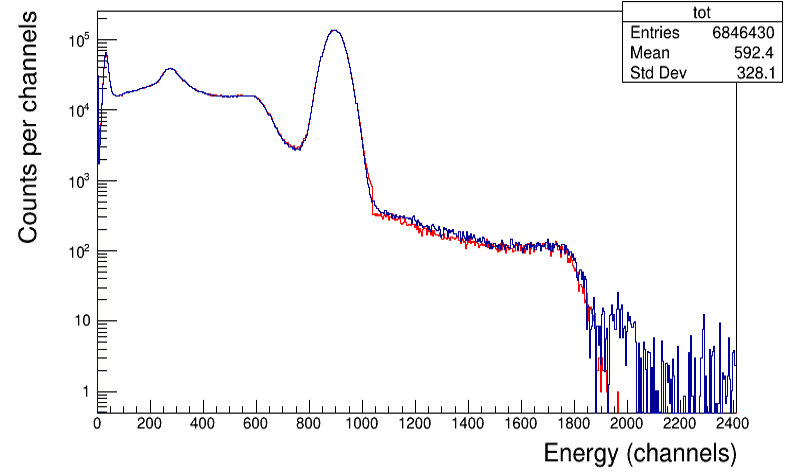
\includegraphics[width=0.78\textwidth]{PileUpTuningThesis.png}}
	\caption{The tuning of the pile-up.
		 The input spectrum is in blue.
		 It was sampled up to 1000 channels.
		 The generated spectrum is in red.}
	\label{fig:pileuptune}
\end{figure}

\section{Fitting Procedure}
The simulation described above were only part of what was needed.
Other simulations included in the fit had the phase space times corrections times or divided an additional factor of the total energy of the electron.:wq:
The simulations were all convoluted and filtered as described above.

\subsection{Data Processing}
The data was processes from the TTrees described in the previous section.
The energy spectrum of the implant detector was put in coincidence with the 4 gamma detectors.
The energy cuts of the gamma detectors were the same as in the life-time measurement.
There was a time difference condition as well.
For this measurement, the time difference between a beta event and a gamma event had to be between -300 and 24 ns.
Then, a 2-D histogram was built, with energy on one axis and time since last beam on on there other.
Since afterglow causes an effect that looks like a gain shift, different time cuts of equal statistics were taken from this 2-D histogram. 
These time cuts were then fit. 
The gain was left as a free parameter to counteract this afterglow effect.

\subsection{Fit Function}
The fit function used was as follows.
First, the x axis of the data was read.
This number was in ADC units, so equation \ref{eq:cal} was used to turn this number into energy in keV.
For the fitting, the gain $G$ was left as a free parameter, but the offset $b$ was set from the calibration.

\begin{equation}
	H(E) = A * (f(E)_{nosum} * S(E,b_{wm}) + f(E)_{summing}) + B*p(E)
	\label{eq:betafit}
\end{equation}

where $A$ is the normalization, $B$ the level of pile-up, $E$ the energy, $b_{wm}$ the weak magnetism, $S(E,b_{wm})$ the shape factor, $f(E)_{nosum}$ the output of the GEANT4 simulation without any energy summing between the ga:
Gamma and beta, and $f(E)_{summing}$ the output of the GEANT4 simulation with energy summing.
The free parameters here are $A$, $B$, and $b_{wm}$.

\subsection{Determining Offset for Shape Fit}

Initially, the offset used was the offset from the calibration  in equation \label{eq:cal}.
The offset used was 10.05 ADC units.
This calibration was determined using photons instead of electrons.
Electrons generate 2\% less light than photons \cite{REFHERE}
This means that the offset found from this fit is suspect to apply to our electron shape measurement.

When applying an offset of 10.05 in a fit of the data, it was found that the output varied greatly as a function of where the fit was started.
This is seen in figure \ref{fig:LBCvbwm}.

%\begin{figure}[!htb]
%ADD FIGURE OF LBC v bwm here

While investigating this effect, several different potential causes were investigated.
The first is if the facator $A$ iin equation \ref{eq:convo} used in to convolute the detector simulation was not the same as the actual detector resolution.
To test that, a Monte Carlo simulation was written.
The space space in equation \ref{eq:phase_space} was multiplied by the shape factor in equation \ref{eq:shapefactor}.
This function was sampled $10^{9}$ times twice to build two histograms. 
Both histograms had a detector resolution applied as described in section \ref{sec:convolution}
One histogram was sampled a turther $10^{6}$ times 10 times to build a sample data set.
The other convoluted histogram was used to fit the generated data set.
The first histogram's $A$ was fixed, while the second histogram's $A$ was adjusted.
When the sample data's $A$ matched the $A$ that were used, no dependence of $b_{wm}$ on the start of the fit.
When the $A$ of the data sample and the $A$, the first thing that happened was that the $b_{wm}$ changed.
If the $A$ differ by a factor of 2 or more, a shift in $b_{wm}$ appears.
However, $A$ was determined to 10\% (FIX)
Having a wrong $A$ cannot explain the effect seen in \ref{fig:LBCvbwm}

The largest effect comes from having the wrong offset in the calibration.
A similar Monte Carlo was written where no convolution was applied.
Sample histograms were generated directly from an analytic function instead of a histogram.
These histograms were generated with an offset of 10 ADC units.
Then, the fit function had a different offset applied to it.
For example, fitting the histogram generated with an offset of 10, and fit with an offset of 20 gives an effect as seen in \ref{fig:MCoffset10applied20}.
This is on the same order of magnitude as the effect we see in the data in figure \ref{fig:LBCvbwm}.

This effect can be exploited to determine the offset using only electron data, 
The size of the slope induced is linear compared to the offset.
By adjusting the offset and noting the slope of the $b_{wm}$ vs the lower beta cut and plotting against the offset, the location of zero slope can be calculated.
This was done, and the result is seen in figure \ref{fig:offsetvslope} 

Doing this procedure gives an offset of -5.11 ADC units. 

\subsection{Fit method characterization}
To characterize the fitting method, two GEANT4 Monte Carlos were generated.
One had had the nuclear shape factor with the nominal value of $b_{wm}$. 
The other had no shape factor, much like the fitting function.
After applying the gamma filtering to both simulations, the simulation results without the shape factor were used to fit the simulation results with the shape factor.
The gain in these fits was left as a free parameter, and the offset was fixed to a value of 0. 
The spectrum with the shape factor became the pseudo-data spectrum.
To manually check the statistical uncertainty, the pseudo-data spectrum was fluctuated.
Each bin had its content and error read. 
That bin error and content was used to build a Gaussian random number distribution.
This random number distribution was sampled, and a new bin center created.
After doing this to the entire spectrum, the new spectrum was fit.
The resulting $b_{wm}$ was recorded.
Then, $b_{wm}$ was set to 43.3, and the Fierz term fit. 
These fitted terms were saved to a histogram.
This was done 1000 times to get a spread of values.
From this, it was discovered that spline interpolation was the best way to fit the spectra.

The same method was used to see if the fitting method induced a lower beta cut effect or not. 
1000 spectra were generated by scrambling one spectrum over and over.
These spectra were fit from a lower beta cut up to the end point minus 100 keV.
The lower beta cut was varied from 200 keV up to 2 MeV.
From this it was found that this fitting method induced an effect above 1200 keV.
This effect was very large in the measurement of $b_{gt}$.

\subsection{Fit details}
The fit was done run by run.
First a prefit for each section was done to calibrate the energy.
Then, two endpoints in keV were used for the fit.
The fitting function with a fixed offset was fit using a maximum likelihood method.
The resulting $b_{wm}$ was recorded.
For the Fierz term fit, the $b_{wm}$ of $^{20}$F decay (43.4) was applied to the shape factor.
Then, the Fierz term was applied to the no summing spectrum and fit. 

The offset used for the fit was -5.11 channels.
The end points for the calibration pre-fit were 540 channels to 7000 channels.
The calibrated end points were 800 keV to 7500 keV. 
 
\subsection{Systematic effects}
\end{document}